\documentclass[../main.tex]{subfiles}
\graphicspath{{\subfix{../images/}}}

\begin{document}

\begin{newrequirements}
    \begin{todolist}
    \item Actual Design description with pictures 
        and diagrams. E.g., a “wiring diagram” 
        of the implemented hardware can be 
        added. 

    \item Actual images of various modules must 
        be included wherever possible. 
        Otherwise, at least the images of 
        various aspects of the completed design 
        must be shown. 

    \item List the different tools and framework 
        used for the implementation. 

    \item Discuss any novel aspects of your 
        implementation (if applicable). You may 
        link this aspect of your design to the 
        comparison table at the end of 
        literature review and elaborate on the 
        steps taken in achieving these 
        novelties in your design. 

    \item Discuss the challenges encountered 
        during the implementation and how they 
        were addressed. 

    \item You may organize any of the above 
        recommended points as subsections 

    \end{todolist}
\end{newrequirements}

\subsection{Hardware}

\lipsum[1]

\subsection{Reinforcement learning}

The framework that we are proposing facilitates the training of
a Parrot drone to achieve a mission that contains uncertainty
based on an arbitrary distribution. 
In our case, the drone is the Parrot Anafi and 
the mission is to complete a 
mobile target visitation task 
in the shortest time and least energy.
The uncertainty of the mission comes from the initial positions and 
movements of the targets.

The initial positions of the targets are generated from 
a skewed
multivariate normal distribution shown in Fig.~\ref{fig:position-distribution}.
After every episode, new positions are generated.
In addition, their movements consist of eight discrete
actions: forward, backward, left, right,
forward-left, forward-right, backward-left and backward-right.
Each movement lasts for 1 meter, and then a new one is
chosen.
We have made the targets such that they choose to move 70\% 
of the time forward-left and 30\% of the time divided
among the remaining seven movements.

\begin{figure}[!t]
	\centering
	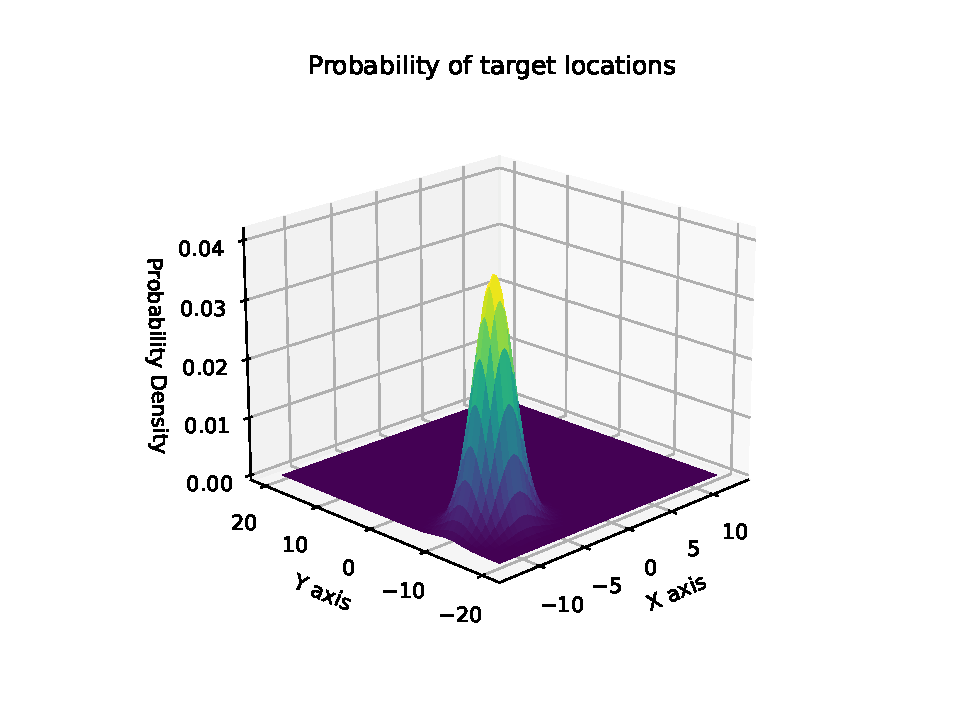
\includegraphics[width=3.4in]{target-distribution}
	\caption{The distribution of the initial positions of the
		targets. The x-y plane corresponds to the ground, and 
		the drone faces the positive x-direction throughout the mission.}
	\label{fig:position-distribution}
\end{figure}

To train a drone using RL requires the
design of the environment, the agent itself and
the interaction between them as shown in Fig.~\ref{fig:rl}. 
The agent, due to being in a certain state, chooses and 
performs an action on
the environment resulting in the environment 
rewarding the agent for taking the action in that state
and then replying to it with a next state.

\begin{figure}[!t]
	\centering
	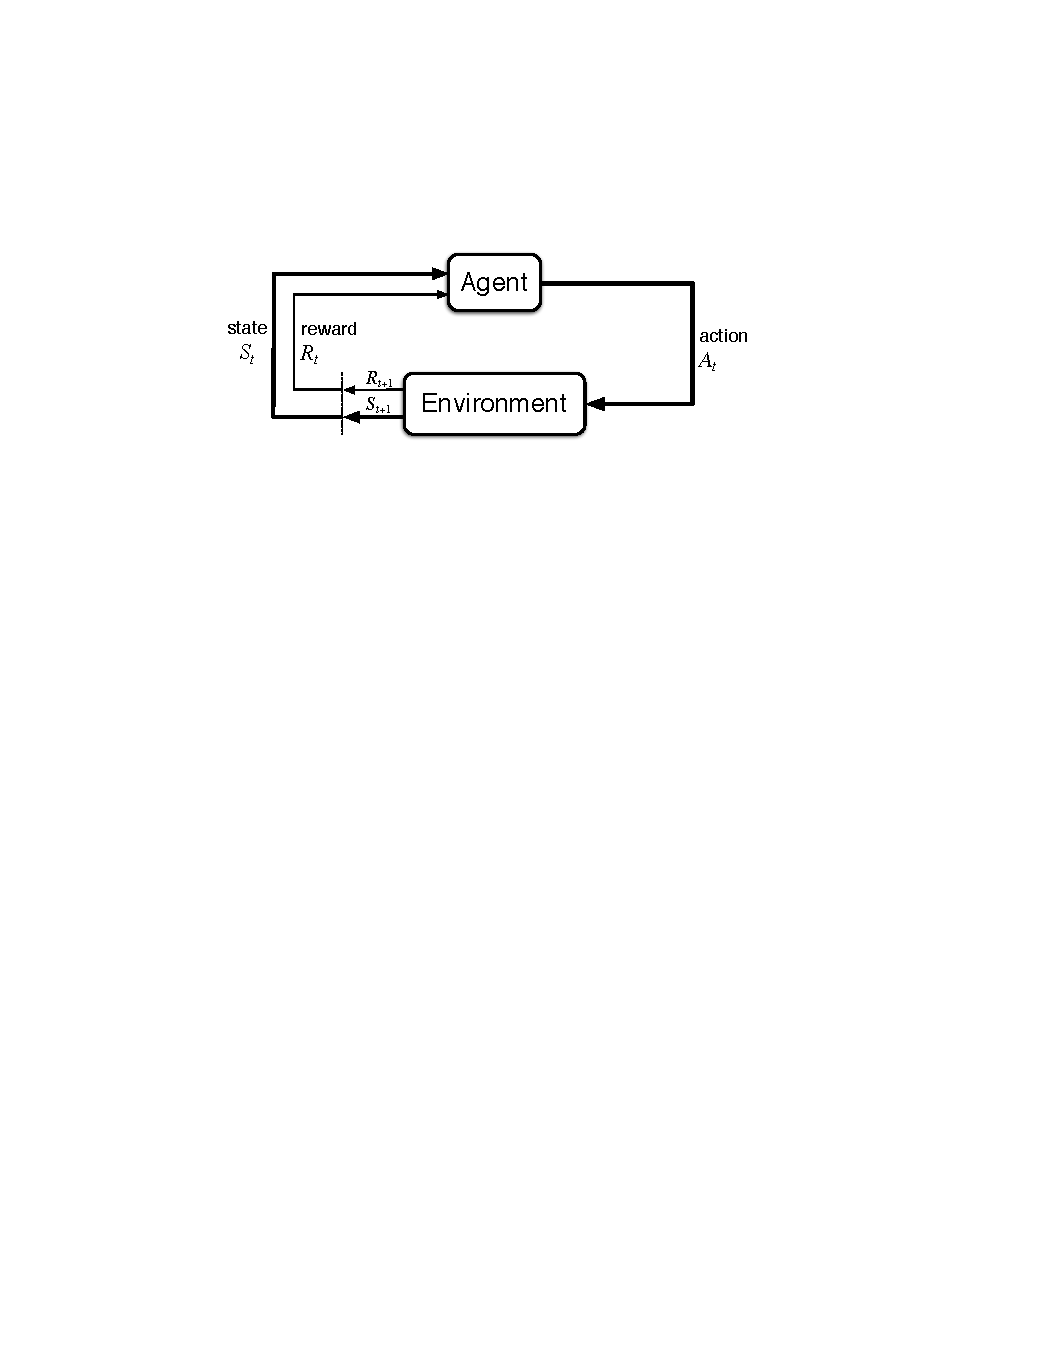
\includegraphics[width=3.4in]{rl-flowchart}
	\caption{The interaction between the agent and environment
		in reinforcement learning \cite{Sut20}.}
	\label{fig:rl}
\end{figure}

In our framework, we have used the Parrot Sphinx simulator
as the environment and a simulated Anafi drone as the agent.
The simulated drone extends the OpenAI Gym \texttt{Env} 
Python class
to inherit the methods every RL agent
needs to undergo to learn.
The exchange of state, reward and action between them 
occur through the Parrot Olympe controller as well as
through JSON-RPC and message passing protocols.
More detailed commands used and steps taken are laid out 
in Fig.~\ref{fig:flowchart}.

\begin{figure}[!t]
	\centering
	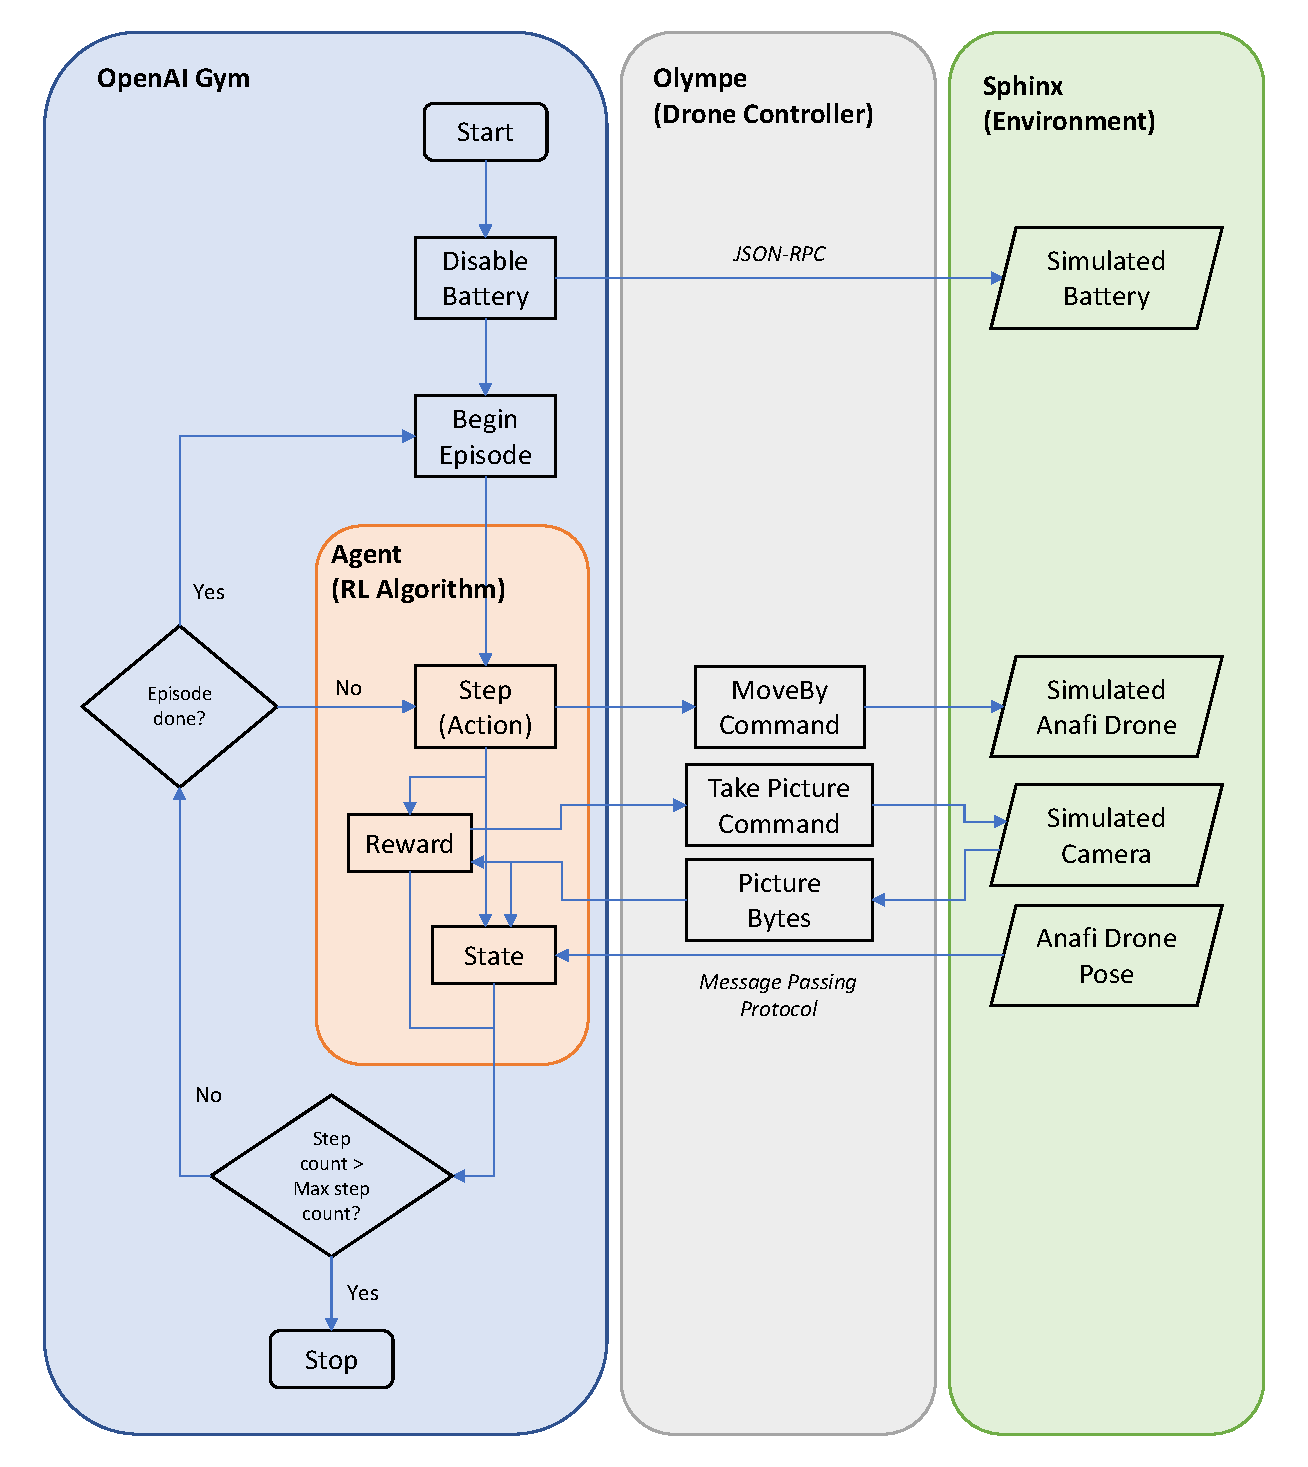
\includegraphics[width=3.4in]{sim-flowchart}
	\caption{Algorithm implementation: commands and messages passing
		between programs to train the drone.}
	\label{fig:flowchart}
\end{figure}

The correct reward and state representations are critical
to making the drone learn to visit the targets in the shortest
time and with the least energy.
The ground is divided into 25 cells as illustrated in 
Fig.~\ref{fig:grid}, and in each timestep,
the drone can occupy only one of those cells.
In addition, each target is given a unique ID which 
is embedded in the QR code that the targets are covered with
as shown in Fig.~\ref{fig:target}.

The drone has nine discrete actions, the first eight of which
are similar to the targets.
They are forward, backward, left, right,
forward-left, forward-right, backward-left, backward-right
and hover. 
Another difference between the drone and target movements 
besides the hovering action  
is the distance travelled -- while the targets move for 
1 meter before changing direction, the drone moves to 
one of the neighbouring eight cells or,
in case of the hovering action, the current cell.

\begin{figure}[!t]
	\centering
	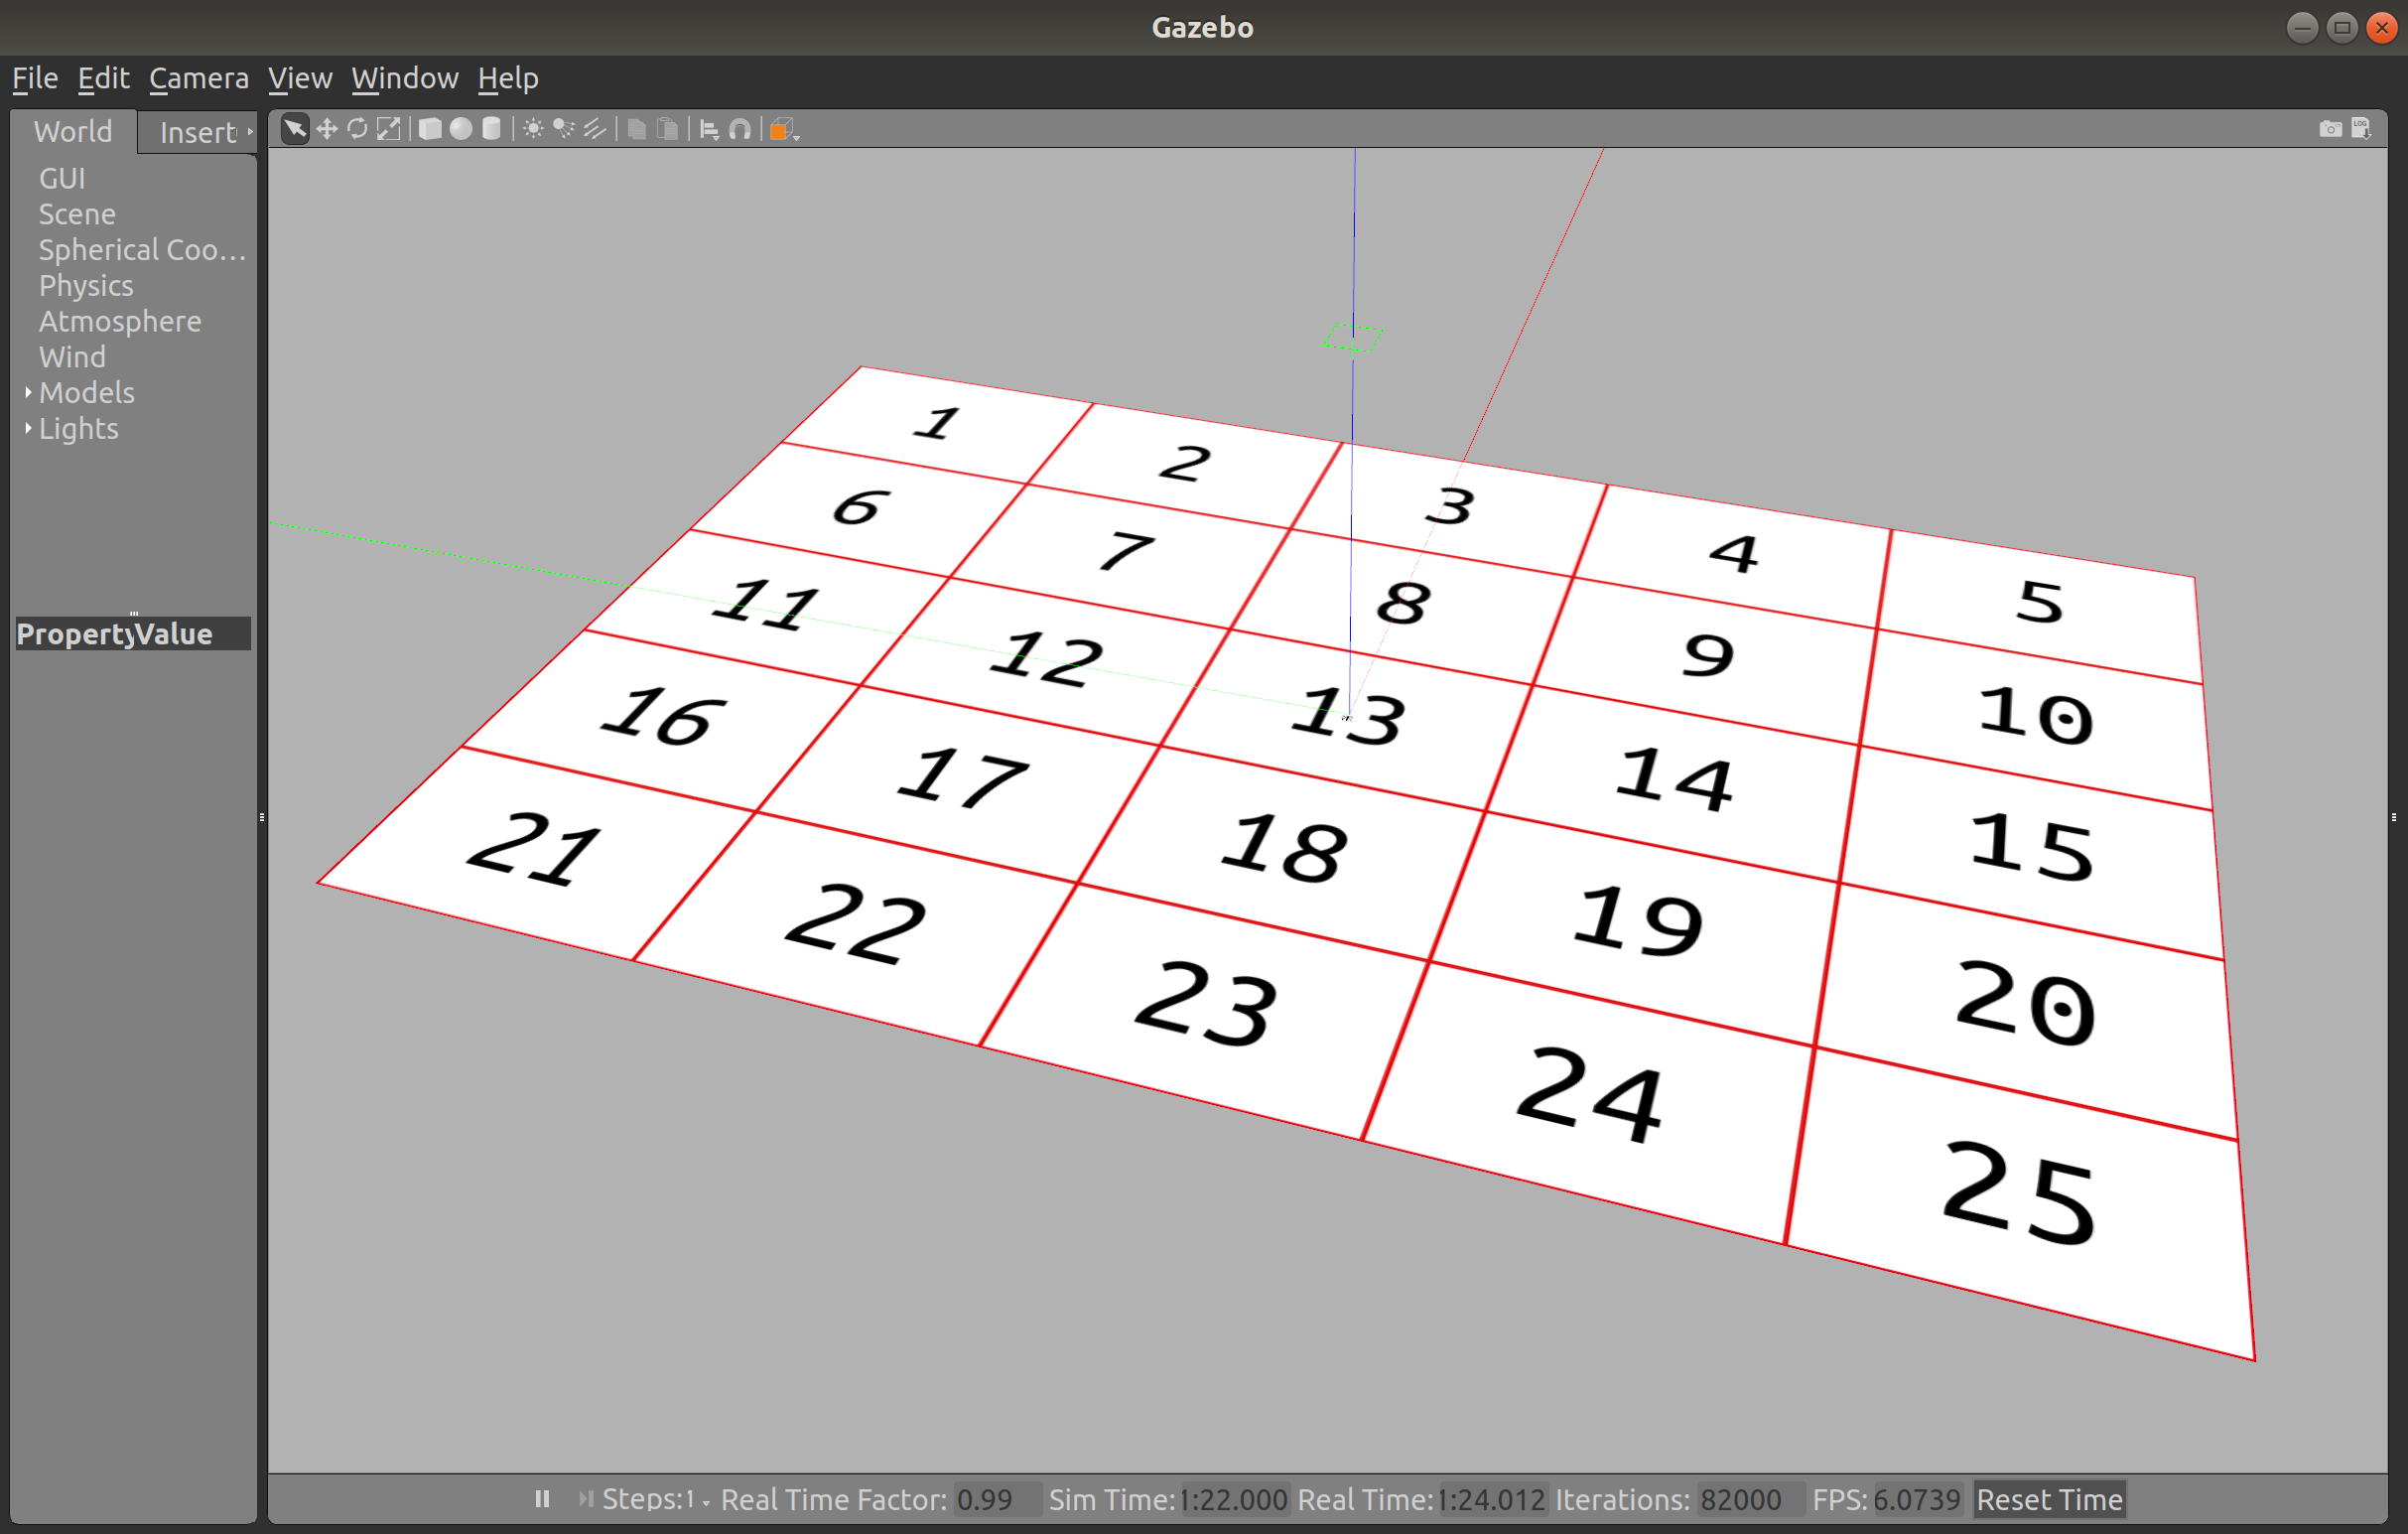
\includegraphics[width=3.4in]{grid}
	\caption{The environment of the agent with its ground
		divided into 25 cells.}
	\label{fig:grid}
\end{figure}

\begin{figure}[!t]
	\centering
	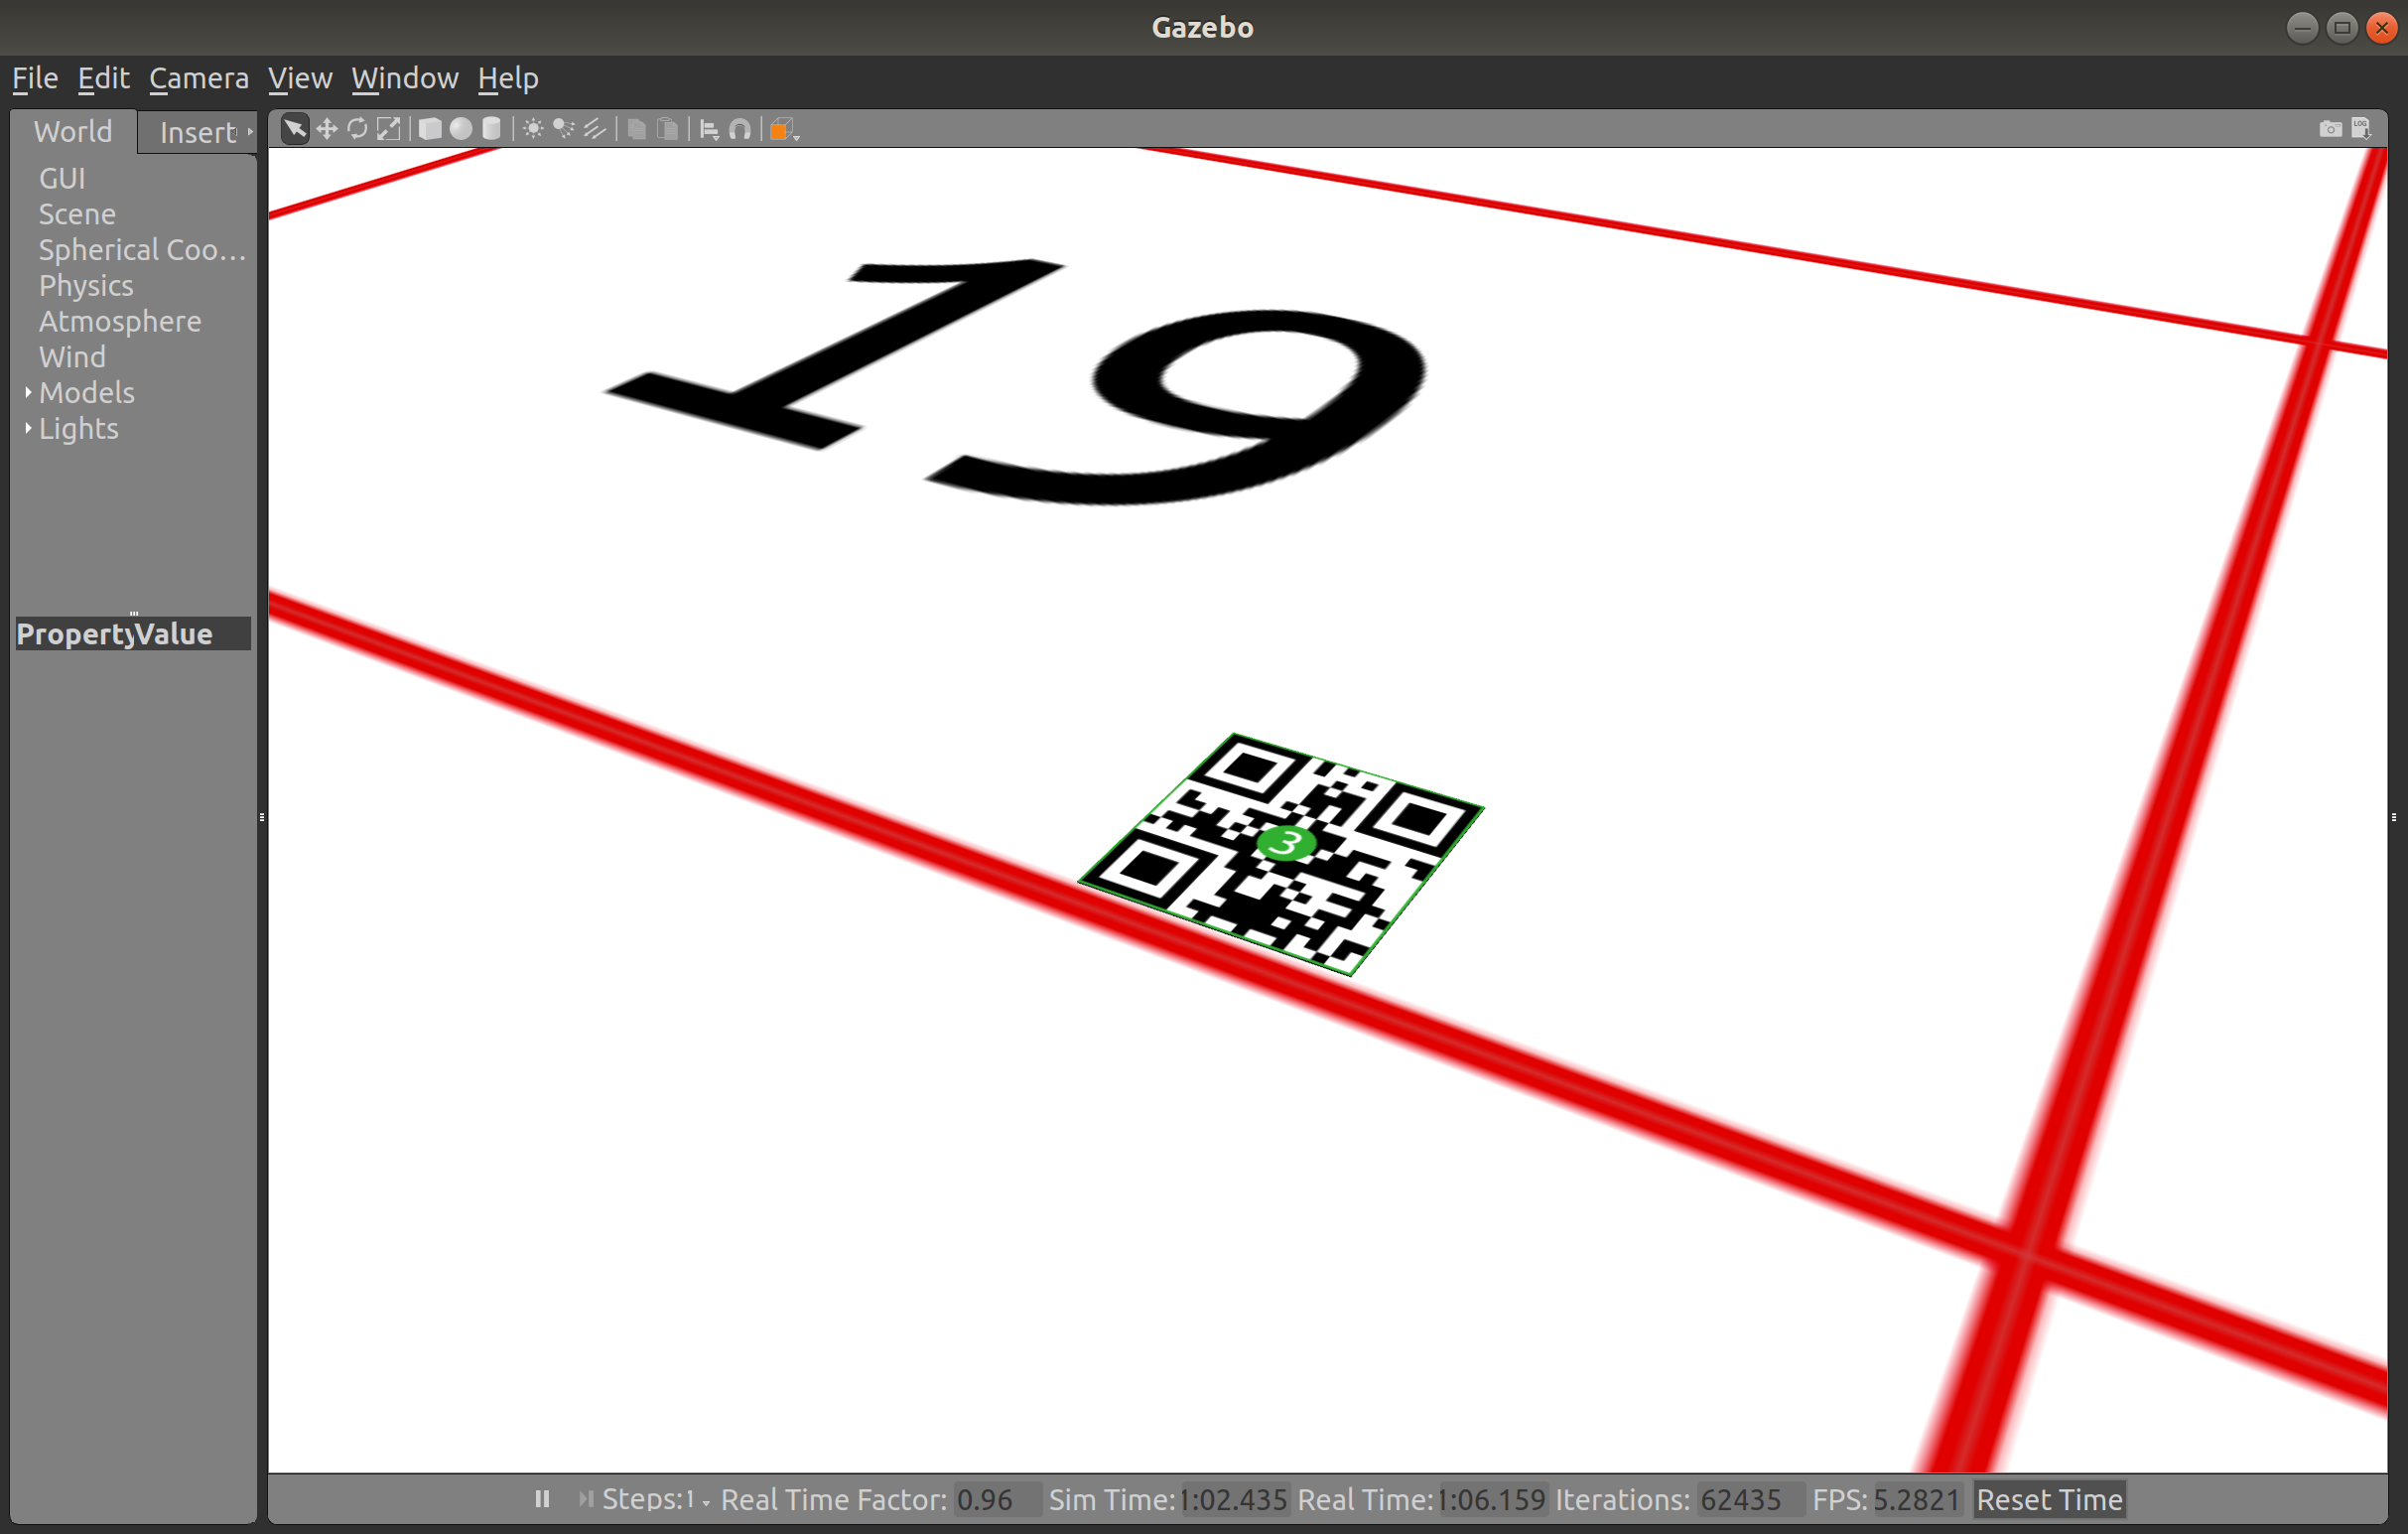
\includegraphics[width=3.4in]{target-3}
	\caption{Example of a target with ID 3 in the environment. The QR code
		embedding the ID information covers the top side of the target.}
	\label{fig:target}
\end{figure}

We have set the reward to be equal to 1.5 multiplied by 
the number of new targets captured in the new state.
If there is no new target, the reward is -1. 
This ensures the drone learns to
minimise the time.
Since there are 10 targets, it follows that the maximum
return (sum of rewards in an episode) that the agent can gain  
in an episode is 15.
To obtain the number of new targets, the drone's simulated camera is
used to take a photo of the cell
underneath, which is then processed by a QR code detection 
model, Pyzbar. 
The outputs of the processing are the IDs of 
the detected targets, 
of which only the previously not encountered ones during 
the episode are counted towards the reward.

On the other hand, the state space is made up of several 
pieces of information as follows
\begin{align}
	s = \{ t, cell, [ I_1, I_2, I_3, \ldots, I_m] \} 
	\label{eq:state-space}
\end{align}

\noindent 
where $t$ is the current time step, $cell$ is the ID of the
cell underneath the drone, $I_k$ is the binary variable 
that indicates if the target with an ID of $k$ has been
visited, $m$ is the total number of targets,
and the vector of length $m$ is the container for the
$I$ indicators. 
For example,
if only targets with ID's 3 and 7 have been visited
in the current and previous time steps since the beginning of the 
episode,
then the vector will have elements of one for $I_3$ and $I_7$ while
the other elements are zeros.

\subsection{User interface}

\lipsum[1]

\end{document}
